\newpage
\section{Experimentación}\label{sec:experimentacion}

En esta seccion se presentaran los resultados de la experimentacion realizada. Pero previamente es necesario conocer los algoritmos con los cuales se comparo nuestra metaheuristca.

\begin{enumerate}
\item Scip: Este algoritmo esta realizado con programacion lineal entera y se explica en detalle en la seccion \textbf{Programacion Lineal Entera}.
\item Goloso: Este algoritmo es un simple Goloso, es decir, en cada iteracion agrega a la solucion en pad que mas ogip tape.
\item Goloso Maximos Locales: Este algoritmo, en cada iteracion busca el pad de mayor ogip (al igual que el goloso), pero como esto esta ligado a la discretizacion, a este pad se lo mueve tratando de ubicarlo en algun lugar cercano donde tenga mayor ogip, es decir, no importa al 100\% la discretizacion, dado que se consigue un pad centrado en la discretizacion (este pad es el pad con mayor ogip de todos los pads centrados en la discretizacion) y luego busco un maximo local en los alrededores y una vez encontrado lo agrega a la solucion.
Para esto se utiliza un parametro \textbf{Paso Movimiento Pad} que indica el paso que se tiene en cuenta a la hora de mover el pad buscando el maximo local. 
Una vez que no tengo mas pads disponibles puede haber pasado que al mover los pads, no tenga mas pads disponibles de los centrados en la discretizacion, pero si existen huecos donde entran otros, por lo tanto, se \textbf{re-discretiza} el area no tapada hasta el momento, se hace una discretizacion mas fina, y para esto se usa el parametro \textbf{Paso mejora Discretizacion} que indica en cuanto se achica la discretizacion. Luego se vuelve a calcular los posibles pads para esta nueva discretizacion. Notar que solo se discretiza mas fino los sectores no tapados por los pads provenientes de la discretizacion mas gruesa.
Por ejemplo, en las siguientes figuras podemos ver como en la primera el paso de la discretizacion es mas grueso que en la segunda (marcado en rojo). Y tambien podemos ver como la discretizacion en la segunda solo se hace en los luegares no tapados. Notar que la discretizacion esta marcada con puntos en la region.

\begin{center}
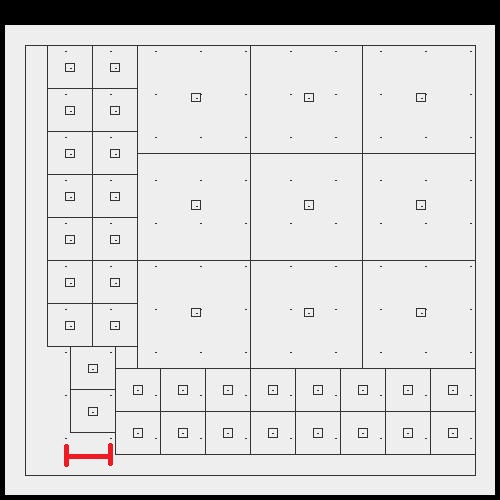
\includegraphics[width=0.4\textwidth]{imagenes/iter40}
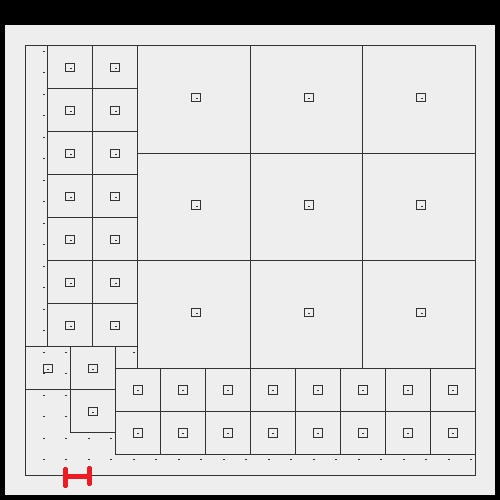
\includegraphics[width=0.4\textwidth]{imagenes/iter45}
\end{center}

\end{enumerate}


Antes de continuar se explican que son cada item de los resultados obtenidos:

\begin{enumerate}
\item Tiempo: 
\item Cant. Pads
\item Area (\%)
\item Ogip
\item Area Superpuesta (del total cubierto) (\%)
\item Cant. Ar. Cubierta
\item Cant. Ar. Superpuesta
\item Ar. Region
\item Iter. Sol.

\end{enumerate}

				

Lo primero que se hizo fue un analisis de la variacion de los parametros. Entonces analizando los resultados en la seccion \textbf{anexo} se concluyo que los parametros CITF (Cantidad Intentos de Tapar una Feromona), FCF (Factor Cambio Feromona), IMPSR (Intentos Meter Pad Solucion Random) se van a dejar fijos. Por otro lado, se decidio hacer que CSRI = CSNRPI dadol que no importa que iteracion sea, siempre dajamos seteada la cantidad de soluciones en un mismo valor. 

Entonces los parametros que nos quedaron para variar son CSRI (Cantidad Soluciones Random Iniciales = Cantidad Soluciones No Random Por Iteracion) , CI (Cantidad de Iteraciones), MCBS (Modo Chequeo Buena Solucion), DF (Discretizacion Feromona)

A la hora de analizar el tiempo vemos que el parametro MCBS no influye, por lo tanto no lo tenemos en cuenta para esta experiemtancion (Nota, se puede ver que el tiempo cambia levemente si se cambia el MCBC, pero nada significativo). 

Lo primero que se analizo fue el tiempo de ejecucion si se varia la cantidad de soluciones por iteracion, y para eso observemos la siguiente tabla:

\begin{center}
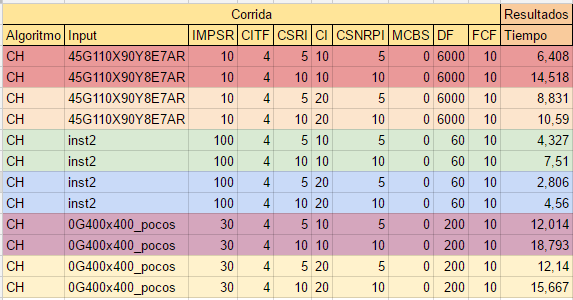
\includegraphics[width=0.4\textwidth]{imagenes/tabla1}
\end{center}

En esta tabla podemos observar 6 subconjuntos de resultados agrupados entre si, donde para cada subconjunto, todos los parametros se mantienen igual excepto la cantidad de iteraciones que varia entre y 5 y 10 (parametros CSRI y CSNRPI). Se puede ver que en todos los casos el tiempo aumenta considerablemente al aumentar la cantidad de soluciones por iteracion, en particular, se puede ver en el primer caso (filas rojas) que al duplicar la cantidad de soluciones por iteracion, el tiempo aumenta a mas del doble (pasa de 6 a 14 segundos).

Observemos que pasa con el algoritmo de colonia de hormigas version 2:

\begin{center}
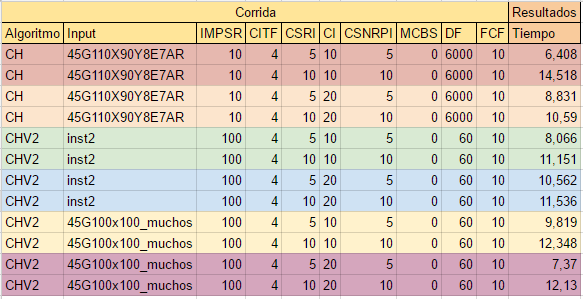
\includegraphics[width=0.4\textwidth]{imagenes/tabla2}
\end{center}

En esta tabla podemos observar lo mismo que en el caso anterior, es decir, al aumentar la cantidad de soluciones el tiempo aumenta. Pero vale destacar que en instancias como \textbf{inst2}, que es una instancia pequenia, el tiempo aumenta poco.

Todos estos resultados tienen sentido, dado que, sin importar la version que se utilice del algoritmo, para cada solucion encontrada tenemos que aumentar la feromona, y la logica de actualizacion de feromona demora bastante, mas alla del tiempo que demora en conseguir la propia solucion. 

A continuacion vamos a analizar que pasa con el tiempo al variar el otro parametro, que es el CI (Cantidad de Iteraciones). 

\begin{center}
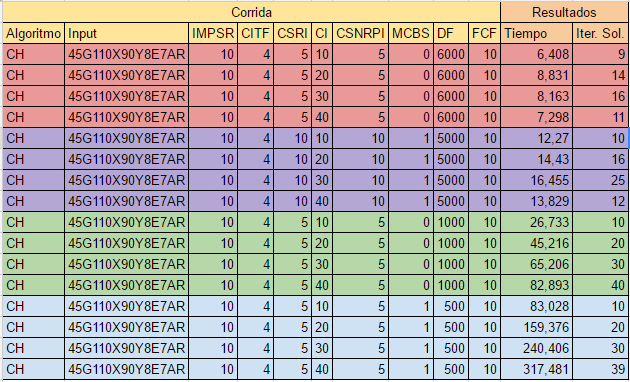
\includegraphics[width=0.4\textwidth]{imagenes/tabla3}
\end{center}

En esta tabla se pueden ver 4 subconjunto de corridas (rojo, violeta, verde y azul). Veamos a continuacion, como se refleja esto en una grafico de lineas.

\begin{center}
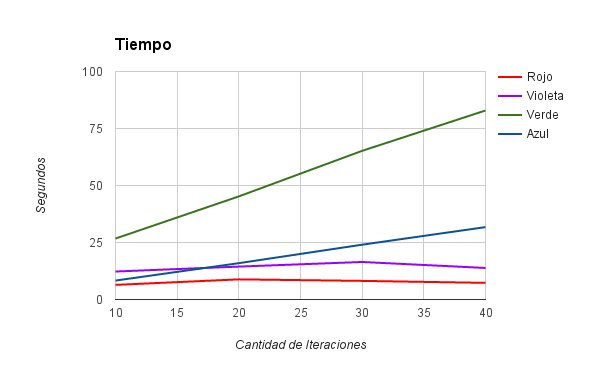
\includegraphics[width=0.4\textwidth]{imagenes/grafico1}
\end{center}

Podemos ver tanto en la tabla como en el grafico, que a medida que aumentamos la cantidad de iteraciones, aumenta el tiempo, excepto en el caso del rojo y violeta. Esto es a causa del que el tiempo, es el tiempo hasta encontrar la mejor solucion y si miramos con detalle la columna Iter. Sol., vamos a observar que en los dos casos que el tiempo disminuye es porque la mejor solucion se encontro antes que los casos anteriores. Este resultado es un resultado correcto, dado que puede pasar que la solucion se encuentre antes ya que cada solucion es distinta de las otras y ademas se comienza con soluciones randoms. 
Por lo tanto vemos que no siempre aumentar la canitad de iteraciones es bueno para mejorar el tiempo ya que encontramos casos donde aumentamos las iteraciones y se tardo mas, pero por otro lado encontramos casos donde aumentamos las iteraciones y se tardo menos y vale aclarar que existen casos donde se aumento la cantidad de iteraciones y la solucion se encontro en un numero de iteracion que era posible encontrar en casos anteriores.

Nota: en el grafico los valores muy elevados se normalizaron (se lo dividio por 10) para que el grafico quede prolijo.

Veamos ahora que pasa usando colonia de hormigas version 2:

\begin{center}
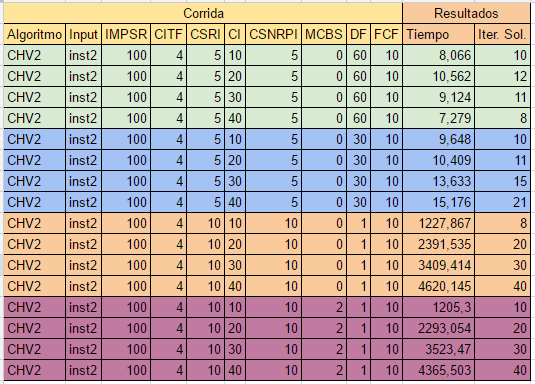
\includegraphics[width=0.4\textwidth]{imagenes/tabla4}
\end{center}

En esta tabla se pueden ver 4 subconjunto de corridas (verde, azul, naranja y violeta). Veamos a continuacion, como se refleja esto en una grafico de lineas.

\begin{center}
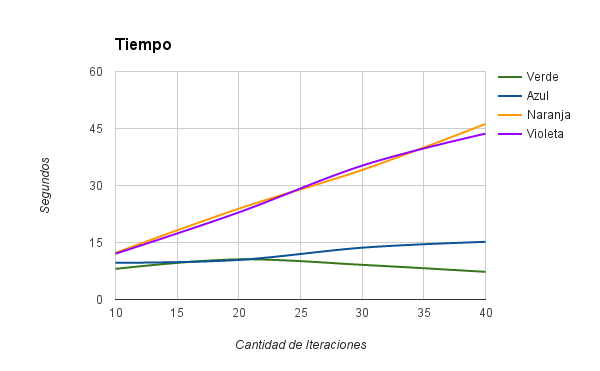
\includegraphics[width=0.4\textwidth]{imagenes/grafico2}
\end{center}

Se puede ver, al igual que en la version 1, que la version 2 se comparta igual, es decir al aumentar la cantidad de iteraciones aumenta el tiempo, pero en algunos casos el tiempo disminiye debido a que la solucion se encontro en una interacion mucho antes.




Agregar comparacion de tiempos para las distintas discretizaciones, es decir, comprar los tiempos de todas las discretizaciones. 



Agregar comparacion de tiempos entre los algortimos, agarrar para cada instancia la mejor soluicion (ogip) y ponerlo todo en una tabla y graficar. Aca se puede explicar mucho. 
Aca se puede charlar que quiza tenemos una solucion no tan buiena pero que tarda mucho mucho menos.


Ahora aca vamos a hacer los esperimentos de ogip.

hacer una tabla variando
CSRI (Cantidad Soluciones Random Iniciales = Cantidad Soluciones No Random Por Iteracion) , CI (Cantidad de Iteraciones), MCBS (Modo Chequeo Buena Solucion), DF (Discretizacion Feromona)
poner 2 ejemplos (2 instancias, los dos algoritmos, es decir, 4 graficos para cada variacion, son 16 graficos).

Ahora aca vamos a hacer el analisis de la feromona, veamos como va variando la feromona

mostrar con picos y sin picos, mostrar con v1 y v2, mostrar la variacion moviendo el MCBS.


